\subsection{Prototyper med fokus på søgefunktionalitet}
\label{subsec:prototype1}
\tjek{Revideret af Elias d. 11.12.12}

Systemets vigtigste funktionalitet er, at brugerne skal være i stand til at udføre en søgning på nogle råvarer, som skal give dem et brugbart resutalt i form af en liste af opskrifter. Uden en søgefunktion er systemet ikke meget værd. Derfor har vi to prototyper, der fokuserer på to forskellige måder, hvorpå man kan udføre en søgning. Den første prototype, som kan ses på \figref{fig:prototype1adesign}, hvor en søgning foretages ved at stave til en råvare, og systemet vil give forslag til, hvilke råvarer, der er søgbare i systemet. 

\begin{figure}[H]
	\centering
	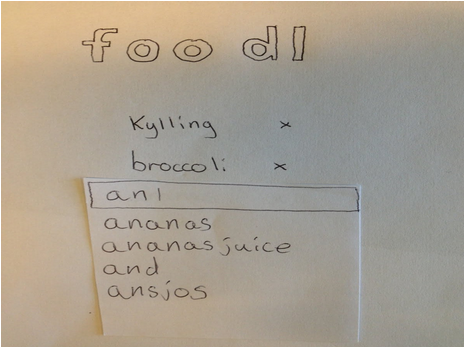
\includegraphics[scale=0.7]{billeder/prototyper/prototype1a.png}
	\capt{Visualisering af prototype 1A, der har fokus på søgefunktionalitet.}
	\label{fig:prototype1adesign}
\end{figure}

Figur \ref{fig:prototype1adesign} minder meget om, hvordan en søgning på \fx Google bliver foretaget. Det er meget minimalistisk. Der er et logo og et søgefelt. Der er blevet foretaget undersøgelser vedr. menneskers hukommelse i forhold til genkendelse af objekter og det at skulle komme i tanke om et objekt. Mennesker er meget bedre til at genkende ting, og det er grunden til, at vi prøver at udvikle en søgefunktion, der minder meget om Googles.\cite[p. ~340]{deb} Google bliver brugt af rigtig mange mennesker, derfor er der en større chance for, at brugere af systemet kan genkende søgefunktionaliteten og derved være i stand til at udføre en søgning uden problemer.

Vi havde kigget på nogle andre eksisterende systemer, der minder meget om vores system. Disse er beskrevet i \secref{sec:eksisterendesystemer}. Herfra fik vi også fået inspiration til en søgefunktionalitet, som vi ønskede at præsentere informanterne for. Denne søgefunktion præsenteres i \figref{fig:prototype1bdesign}, hvor man manuelt skal vælge råvarer fra kategoriserede lister.

\begin{figure}[H]
	\centering
	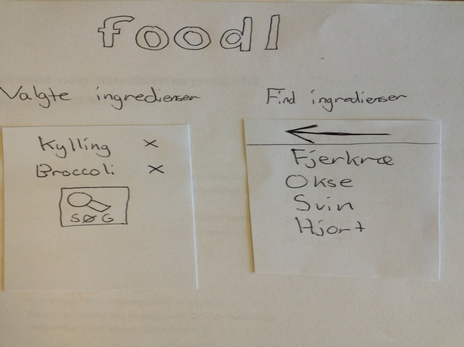
\includegraphics[scale=0.7]{billeder/prototyper/prototype1b.png}
	\capt{Visualisering af prototype 1B, der har fokus på søgefunktionalitet.}
	\label{fig:prototype1bdesign}
\end{figure}

Figur \ref{fig:prototype1bdesign} præsenterer brugeren for to vinduer, hvor man i det venstre vindue kan se, hvilke ingredienser, man har valgt, og man vælger nye ingredienser i det højre vindue.

Begge informanter var enige om, at prototypen i \figref{fig:prototype1bdesign} virkede mere rodet og meget mindre intuitiv end prototype 1A, som mindede om Googles søgefunktion, som vises i \figref{fig:prototype1adesign}. Begge informanter var enige om, at denne var hurtig, nem og effektiv. Merete havde ikke behov for en kort vejledning før hun begyndte at benytte søgefunktionen.

Informanterne mente begge, at prototype 1B var langsommere at bruge og de syntes ikke om den. Merete var i tvivl om, hvilken kategori hun skulle vælge \fx kylling fra (\fx kød eller fjerkræ?). Kategorierne kan laves på mange forskellige måder, og uanset hvordan de vælges, vil der med garanti være nogle brugere, der vil være i tvivl om, hvor de skal lede efter en bestemt ingrediens.

På baggrund af informanternes feedback, valgte vi at arbejde videre med prototype 1A. I \secref{sec:webapplikationen} introducerer vi brugergrænsefladen for systemet, og den bærer meget præg af vores test med informanterne og disse prototyper.